2048 is a popular solitaire board game available, e.g., online on \url{https://2048.io/}. In this exercise, you are to implement a version of this game in F\# and using \lstinline{Canvas}. The rules, you are to implement are as follows:
\begin{enumerate}
\item The board is a square board with $3\times 3$ field.
\item The pieces are colored squares: red, green, blue, yellow, black corresponding to the values 2, 4, 8, 16, 32.
\item There can at most be one piece per field on the board.
\item The initial conditions is a red and a blue piece placed on the board.
\item The game can be tilted left, right, up, down by pressing the corresponding arrow keys.
\item When the game is tilted, then all the pieces are to be moved to the corresponding side of the board.
\item If two pieces of the same color are pushed into each other in the process of tilting, then they are replaced by a single piece of double the value. For example, the board in \Cref{case1a} is tilted to the right, and the two red pieces are replaced with green piece.
  \begin{figure}
    \centering
    \subfigure[\label{case1a}]{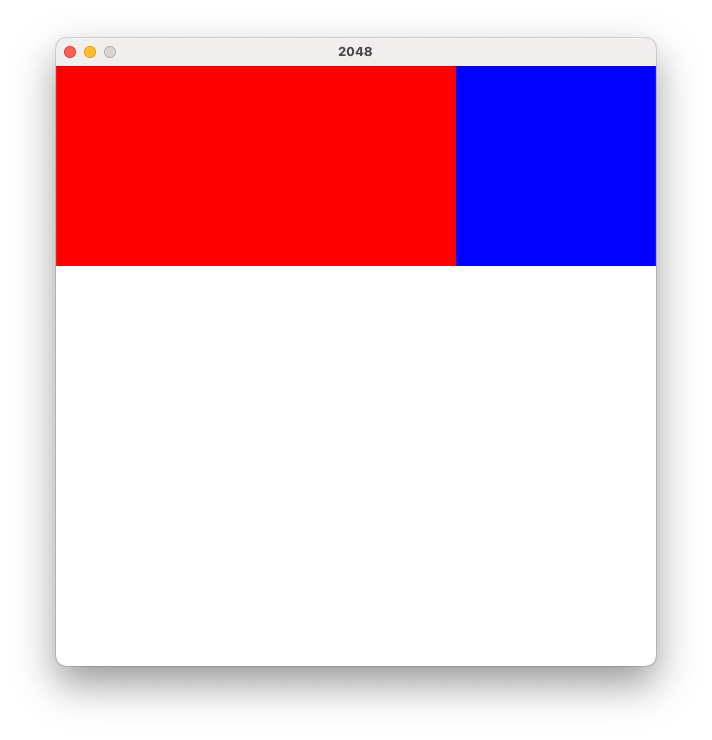
\includegraphics[width=0.22\textwidth]{case1a.png}}
    \subfigure[\label{case1b}]{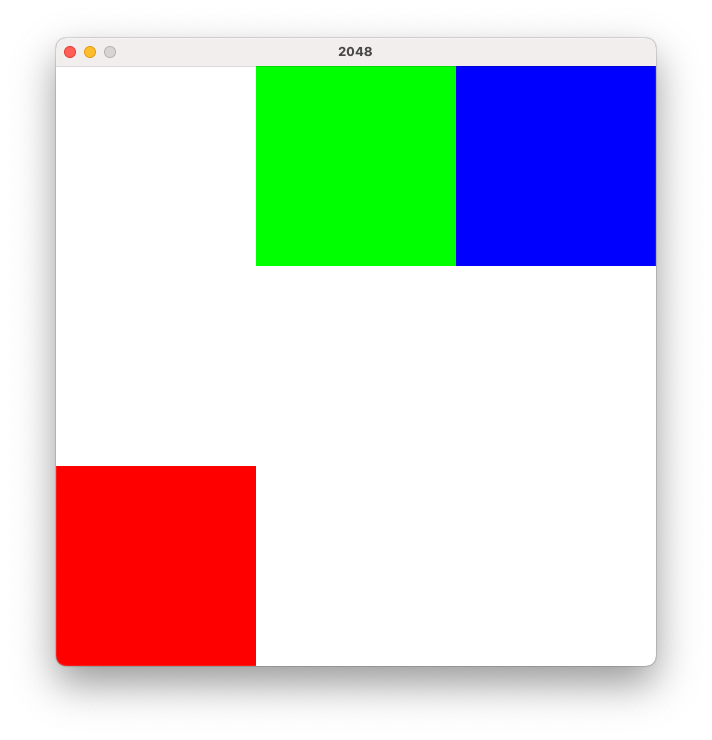
\includegraphics[width=0.22\textwidth]{case1b.png}}
    \subfigure[\label{case2a}]{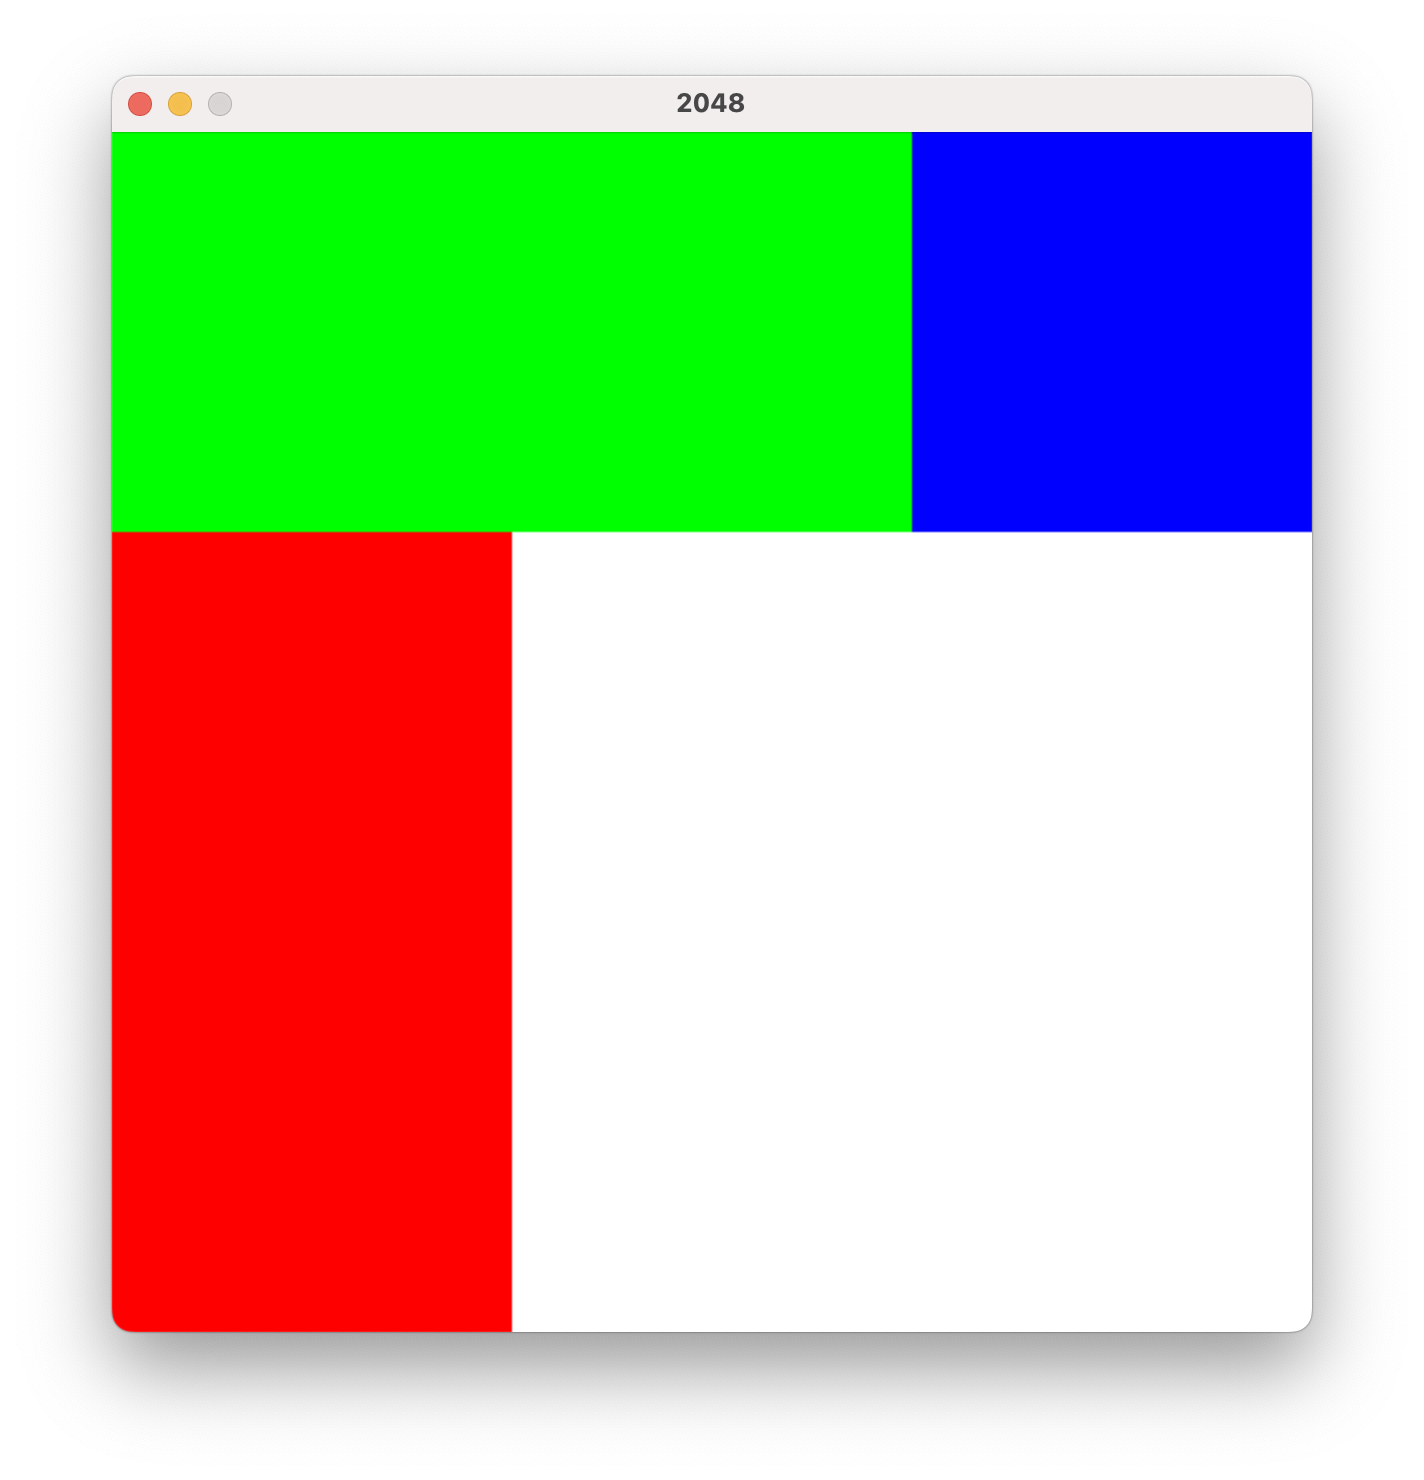
\includegraphics[width=0.22\textwidth]{case2a.png}}
    \subfigure[\label{case2b}]{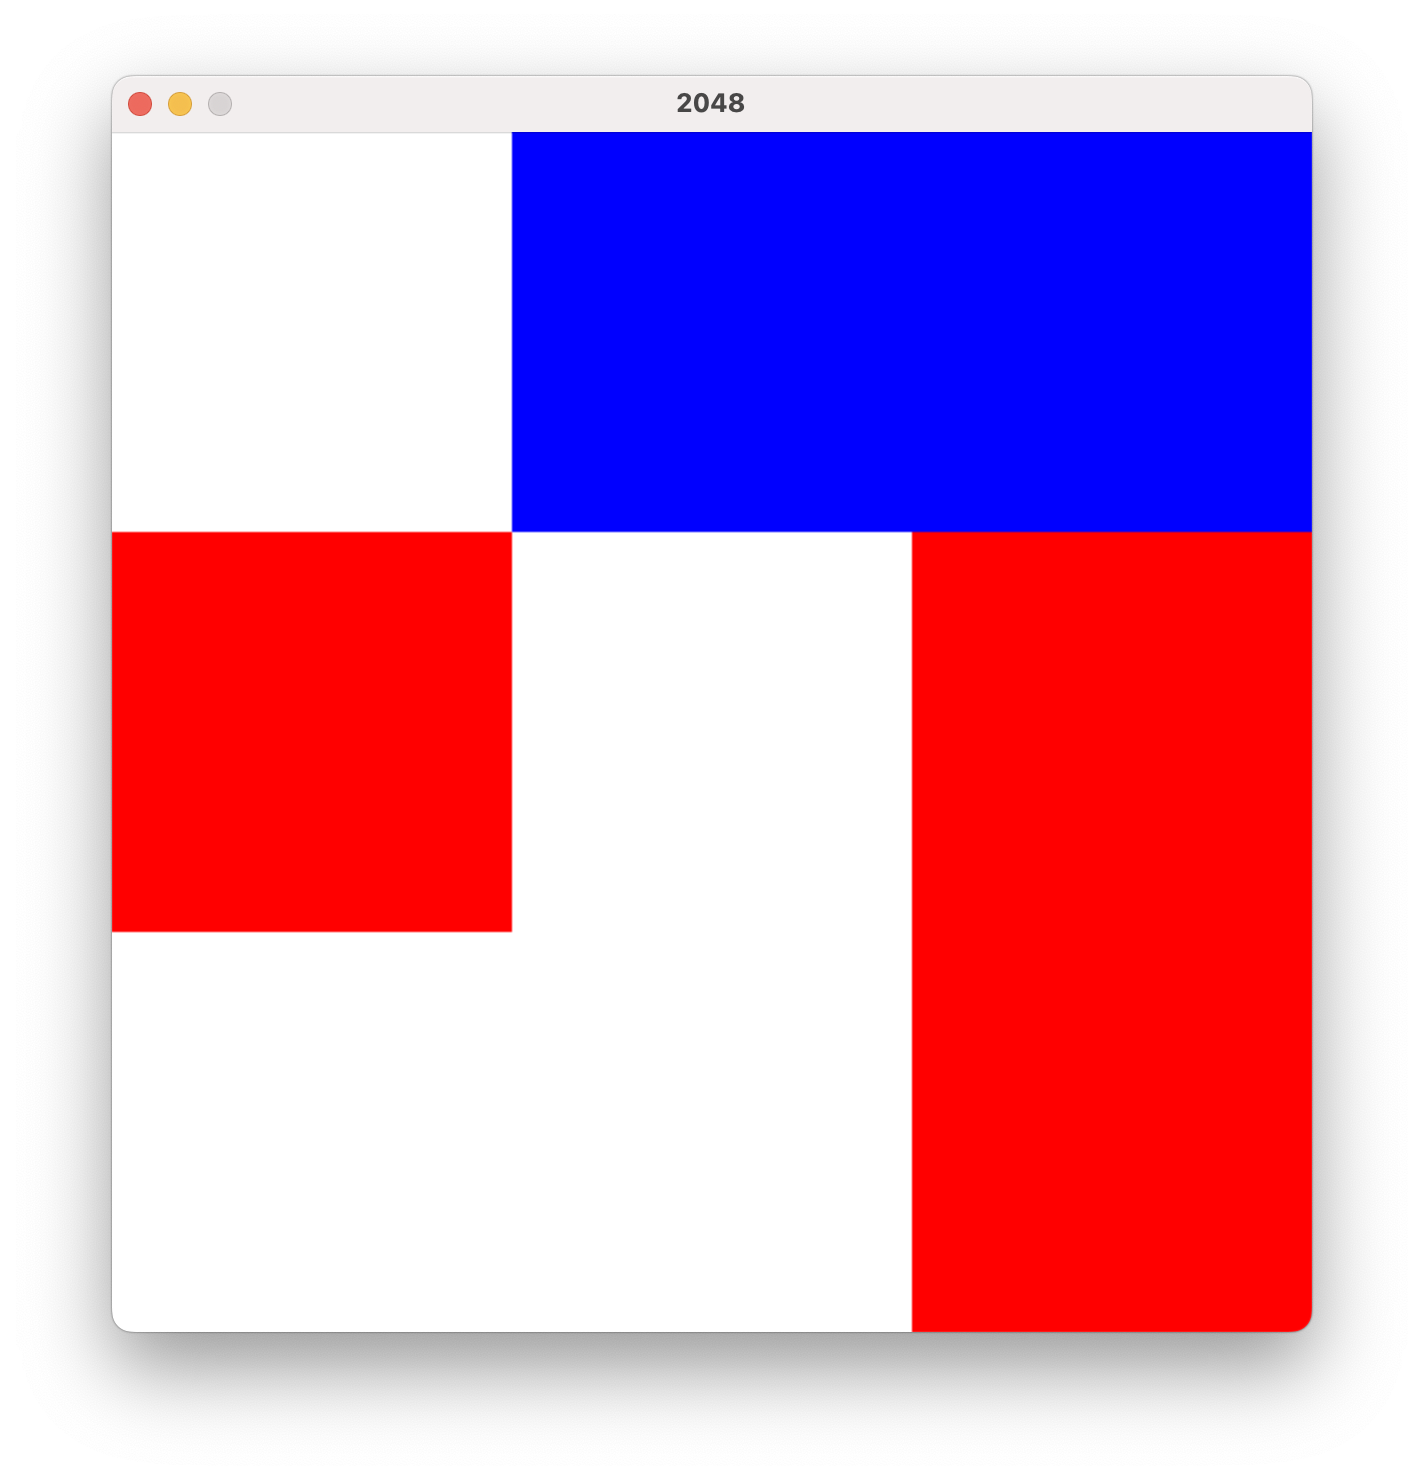
\includegraphics[width=0.22\textwidth]{case2b.png}}\\
    \subfigure[\label{end}]{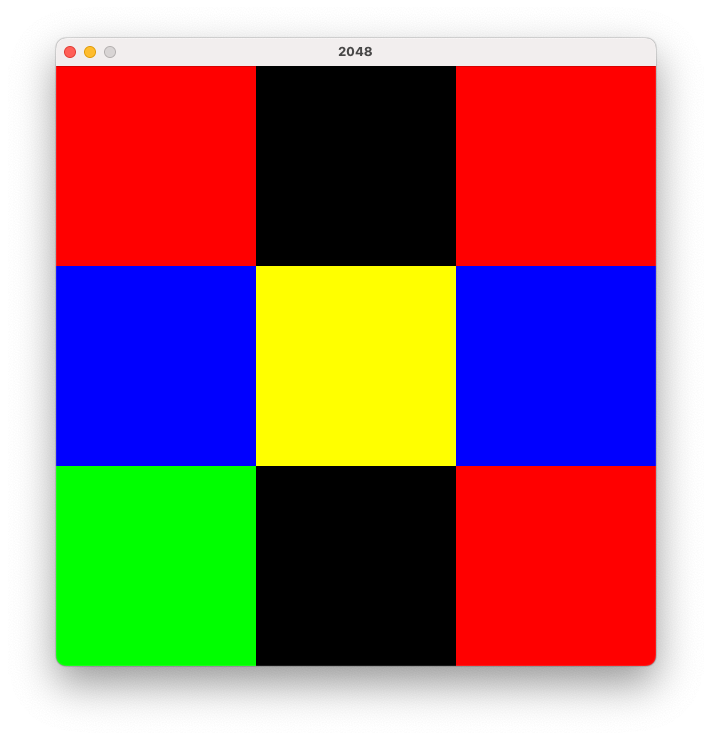
\includegraphics[width=0.22\textwidth]{end.png}}
    \caption{Some examples}
    \label{fig:2048Samples}
  \end{figure}
However, replacement is not performed in a cascading fashion, e.g., the board in \Cref{case2a} is tilted to the right combining the two green to a blue, but the resulting two blues are not combined.
\item Two black pieces are combined into one black piece.
\item After each turn, a new red piece is to be placed randomly on an available field on the board.
\item The game ends when there are no possible moves and no empty locations for a new piece to spawn.
\end{enumerate}
In your solution, you are to represented a board with its pieces as a list of pieces, where each piece has a color and a position. This is captured by the following type abbreviations:
\begin{lstlisting}
type pos = int*int // A 2-dimensional vector in board-coordinats (not pixels)
type value = Red | Green | Blue | Yellow | Black // piece values
type piece = value*pos //
type state = piece list // the board is a set of randomly organized pieces
\end{lstlisting}
In the following, the first coordinate in pos will thought of as a up-down axis also called the row, and the second as an left-right axis also called the column with $(0,0)$ being the top-left.